\chapter{Sprint 4}
\label{chap:sprint4}
The following section presents an overview of how we planned, worked and
completed sprint 4.

Sprint 4 started on 15th of October and ended on 28th of October.

The chapter is divided into five parts, starting with the overall plan for the
sprint in Section \ref{sec:sprint4sprintplan}. Followed by the sprint backlog, which
enlists the tasks that have been chosen for the sprint. Section
\ref{sec:sprint4designAndImplementation}.
will focus on the work made to the GUI, the logic implemented in the application and the work done to the database and database access in the application.
The chapter ends with what have been tested and the corresponding results in
Section \ref{sec:sprint4testingAndResults} and a sprint review in Section
\ref{sec:sprint4sprintRetrospective}.

\section{Sprint Plan}
\label{sec:sprint4sprintplan}
The plan for the sprint is to work on a broad spectrum of functionality for the application. 
With four weeks left to work on implementation, and the last week needed for bug fixing and 
wrapping up the code, the time is starting to run out. For much of the user stories it was either make it this sprint or break it, 
since we didn't want to deliever half-finished code.

The general look and feel of both applications was fairly generic and not good-looking. At the start of the sprint, the GUI consisted of mostly standard elements and some pictures we painted ourselves, leaving poor software. Therefore the GUI in both applications were in for a huge upgrade. 

\subsection{CAPP}
During the first customer meeting, we made a decision to remove functional requirement CF4: ``The application should have an avatar for each child, that can be chosen by the child, and
customized through the shop.''. We felt that the shop idea was simply too big of a task to implement during the last four weeks in addition to all the other work that remained. 
The gamification part of the project was now reduced to a showing of amount of rewards a child had collected, and we decided that this reward would be an amount of stars. 
However, we kept the database-tables such that it would we easier to extend the application with this functionality. 


Regarding the reward system of CAPP we decided to make a more visual overview of how many stars are 
collected, since children does not necessarily know how to read. We also had to implement a 
connection between the database and this view.

The distraction was up for refactoring. The solution we had at the start of the sprint was a 
very simple, not very disctracting, countdown. The customer wanted to change this, and 
told us they would create pictures in order to make a better distraction.

Instructions for correct use should also be implemented during this sprint. Since the 
instructions are for children, they are implemented as a picture gallery downloaded froam 
an external server. 

\subsection{GAPP}
To the log of GAPP we plan to implement functionality for registering a treatment which was 
taken earlier, without the app present. We also planned to add a pollen forecast to the 
calendar, as it may warn users about possible pollen spread, since this may effect the child's health state.

To the settings functionality, we planned to improve the general layout of the menu for 
adding a medication plan. Also this part of the application needs to be connected to 
the database, which will be done during this sprint.

To the reminder functionality the plan was to make finishing touches in order to make it work.

\section{Sprint backlog}
This section contains table \ref{tab:sprint4backlog} with the sprint backlog, which is a smaller part of the product 
backlog. The goal is to implement the entire sprint backlog during the sprint.

\begin{table}
	\begin{center}
		\begin{tabular}{|p{2.0cm}| p{7.0cm}| p{2.0cm}|p{2.0cm}|p{2.0cm}|}
			\hline
			\#  ID 	& Task 	& Story points 	& Estimated hours & Responsible \\
			\hline
			1.1 & View for amount of stars collected & 1 & 4 & Yngve\\
			\hline
			1.2 & Connect reward view to the database & 1 & 4 & Yngve\\
			\hline
			2.1 & Refine the distraction for the children & 3 & 12 & Yngve\\
			\hline
			3.1 & Finalize instructions for children & 3 & 12 & Aleks\\
			\hline
			4.1 & Make solution for registering a treatment & 3 & 12 & Esben\\
			\hline
			4.2 & Implement pollenfeed to log & 10 & 40 & Esben\\
			\hline
			4.3 & Finalize view for showing pollen and medications taken at a given day & 2 & 8 & Esben\\
			\hline
			5.1 & Finalize instruction for medications & 3 & 12 & Aleks\\
			\hline
			6.1 & Make view for viewing existing medication plans & 4 & 16 & Eirik\\
			\hline
			6.2 & Import medication list from database to medication plan settings & 1 & 4 & Esben\\
			\hline
			6.3 & Improve layout for making medication plan & 2 & 8 & J\o rgen\\
			\hline
			6.4 & Save the medication plan to the database & 3 & 12 & J\o rgen\\
			\hline
			7.1 & User interface for changing reminder preferences & 1 & 4 & \\
			\hline
			7.2 & Secure that the reminder is giving alarms independently of internet connection and sound level on phone & 1 & 4 & Eirik \\
			\hline
			8.1 & Create web interface page for adding medical plan doses & 1 & 4 & Yngve \\
			\hline
			8.2 & Create web interface page for removing medical plan doses & 1 & 4 & Yngve \\
			\hline
			8.3 & Create web interface for getting log grouped on days & 1 & 4 & Yngve \\
			\hline
			9.1 & Refine Karotz app manus, after feedback from customer & 3 & 12 & Yngve \\
			\hline
			9.2 & Record new voice messages for the Karotz & 1 & 4 & Yngve\\
			\hline
			10.1 & Refine design for registering treatment & 1 & 4 & Esben and J\o rgen \\
			\hline
			10.2 & Refine design for instructions & 2 & 8 & Esben \\
			\hline
			10.3 & Refine GUI for the main menu & 1 & 4 & Aleks and Esben \\
			\hline
			11.1 & Refine alarm and distraction regarding database calls & 2 & 8 & Yngve\\
			\hline
			\bfseries{SUM} & & \bfseries{51} & \bfseries{204} & \\
			\hline
			\hline
		\end{tabular}
	\end{center}
	\caption{Backlog for sprint 4}
	\label{tab:sprint4backlog}
\end{table}

\section{Design and Implementation}
\label{sec:sprint4designAndImplementation}
This section will present the changes done during the sprint.

\subsection{User Interface Layer}

\subsubsection{CAPP}
Huge changes were made to the main menu of CAPP. The buttons from earlier were removed, and instead 
all buttons throughout the application is image buttons, meaning it is a picture which works 
as a button when pressed. 

During this sprint we added functionality for viewing instructions in the child application. 
The instructions are accessible from the main menu. Upon opening the instructions the user is 
met with a picture series where the user may view pictures that give information regarding how 
to use the medicines correctly.

The distraction for treatment was given a facelift in form of a huge change-out of the pictures. 
During the sprint we added new pictures and interactive design for the user to interact 
with the Karotz. We also added more sound files, to make it sound like the Karotz is talking 
to the user. 

\subsubsection{GAPP}
During this sprint we added functionality for viewing the pollen forecast for today's date and 
the following day. Using ``Pollenvarslingen", an external API, the application can make calls to an external server 
and recieve an XML-feed in return. This XML-feed gives certain info about the pollen forecast. 
Regarding this there were some problems. Since there is no pollen in the air in October, all 
calls to the API returned empty XML-feeds. After discussing this problem with the customer, we 
found out that we solved this by setting up a dummy XML-feed on our own external server. The 
XML-feed would always return the exact same document, but it still made it look like a real 
pollen forecast.

The main menu of the app was given some changes. The buttons from earlier are gone, and instead 
all buttons throughout the application is image buttons, meaning it is a picture which works as 
a button when pressed. 

During this sprint we added functionality for viewing instructions in the application. The 
instructions are accessible from the main menu. Upon opening the instructions the user is met with 
a picture series where the user may view pictures giving information regarding how to use the 
medicines correctly.

The menu for choosing treatment plan was polished with new images and text, to make it more 
understandable and intuitive. 

The calendar will now show what health state the child was in, by coloring a bar on top of the 
given day. The bottom bar of each day will be colored according to the worst amount of pollen on 
the given day. Since there is no pollen in the winter season, we have hardcoded the values for the 
amount of pollen, which makes the log show no differences between days.

\subsection{Application Logic Layer}
In the menu for the treatment plan, the application will now create reminders based on what 
treatment plan is chosen. Different treatment plans will also affect the amount of stars the 
children will recieve upon finishing a treatment.

The menu for registering a treatment taken earlier, will now save to the database, based on what 
date and what medicine the user chooses from the menu.

The information about medicines will now show a listed menu of the different medicines. When a
medicine is chosen by click, it will load a screen with info from the database.

\subsection{Data Persistence Layer}
The following web access pages were added during the 4th sprint:
\begin{itemize}
  \item \emph{add\_plan\_dose.php:} Inserts a new entry in the \code{MEDICAL\_PLAN\_DOSES} table for the given child, health state a dose 
  		of the given medicine at the given time. This is the primary module used to alter medical plans. Returns the ID of the
  		added dose.
  \item \emph{remove\_plan\_dose.php:} Deletes the entry in the table \code{MEDICAL\_PLAN\_DOSES} which correspons to a given id. Returns
  		the number of deleted rows.
  \item \emph{get\_log\_days\_for\_child.php:} For the calendar in GAPP, it was advantageous to have a database access method that
  		could return a list of days in a month with the child health state for each day, and a list of doses taken on that day.
  		\emph{Get\_log\_days\_for\_child.php} accomplishes this by using the table \code{CHILDREN\_LOG\_DAYS} to find the latest recorded
  		health state before the given month started. Then it iterates through all the days, checking if there are any days in the month
  		where the status changes, and adding all doses, taken from \code{DAY\_MEDICINE\_DOSES}, on that day. The method takes a \code{child\_id},
  		and two optional parameters \code{month} and \code{year}. If the month and year are not set, the values for the current days
  		are used.
  \item \emph{remove\_plan\_medicine\_at\_time.php} During development of the adult app GAPP, it was discovered that using a
  		combination of \code{child\_id}, \code{medicine\_id} and \code{time} as the key for removing elements in the \code{MEDICAL\_PLAN\_DOSES}
  		table would be easier than using an ID. Therefore the need for this module arised, and it simply removes all entries in the
  		table that fit the criteria.
\end{itemize}

Changes were made to the following files for web access:
\begin{itemize}
  \item \emph{add\_child.php:} Since we moved away from the avatar idea, this method no longer creates an entry in the \code{AVATARS} table, and does
  		not return an ID for that entry. 
  \item \emph{set\_child\_state.php:} Now updates the table \code{CHILDREN\_LOG\_DAYS} with the given health state.
  \item \emph{register\_medicine\_taken.php:} Adds the calculated reward to the child's total credits in the \code{CHILDREN} table. If 
  		no time is given, a default time of 00:00:01 is set.
\end{itemize}

The following changes were made to the database itself:
\begin{itemize}
  \item Since the Avatar idea was at least put on hold, there is no need to store credits in the avatar for a 
  		child. An extra column named \code{credits} was therefore added to the \code{CHILDREN} table.
  \item To support several medical plans for a child and to be able to save such plans and change back and forth between them, 
  		a column \code{child\_id} was added to the table \code{MEDICAL\_PLANS}. It is therefore possible to indicate the ``active'' 
  		medical plan with the id in the \code{CHILDREN} table, but many can be stored to a child. Subsequently the useless \code{label} 
  		column was dropped. 
\end{itemize}

\subsection{Karotz}
The sound clips for the Karotz were changed in order to be more understandable for children. We had simply not thought of aspects 
such as the Karotz should count from 0 to 10, since children does not necessarily know how to count backwards. The Karotz will 
now communicate with the database in order to save rewards earned by the user. At the end of this sprint, the Karotz had all 
desired funtionality for reminders, distraction, instruction and rewards. Testing on users still remained, and was planned for 
the beginning of sprint 5.

\section{Testing and Results}
\label{sec:sprint4testingAndResults}

\subsection{Testing}
Table \ref{tab:unit4.1} shows the unit test performed this sprint.

\begin{table}
	\begin{center}
		\begin{tabular}{|p{3.0cm}|p{14.0cm}|}
			\hline
			\bf{Item} & \bf{Description}\\
			\hline
			\bf{ID} & UNIT4.1\\
			\bf{Description} & Test that the right instructions are downloaded and shown on screen in the instructions menu\\
			\bf{Date} & 18. 10. 2012\\
			\bf{Responsible} & Aleks\\
			\bf{Subject} & Medication instructions and external database \\
			\bf{Precondition} & The application is running, the database is running\\
			\bf{Steps} &
			\begin{tabulenum}
			    \item Press Instructions button in the main menu.
			    \item Choose a medication from the list shown.
			    \item Observe if the correct picture is shown on screen
			    \item Observe if the correct text (instructions) is shown on screen.
			\end{tabulenum}\\
			\hline
			\bf{Results} & The first few times, a blank screen was shown. After debugging, all worked as expected. More about this in results\\
			\hline
		\end{tabular}
	\end{center}
	\caption{Unit test 4.1: instructions}
	\label{tab:unit4.1}
\end{table}

\subsection{Results}
Regarding the test UNIT4.1, we had some problems with showing the instructions. The page 
returned a blank screen, regardless of what medicine was chosen. We controlled the 
servers responds by using a browser, to make it easier to read the return values. The 
return values where correct each time.

After extensive debugging, we discovered that the query done in the application was 
written in an illegal way. This way, the query was not parameterized as a query and 
the server did not respond to the request. After fixing the query, everything worked as expected. 

\section{Sprint Retrospective}
\label{sec:sprint4sprintRetrospective}
This section contains an evaluation of the sprint. The evaluation is done mainly by the us, but feedback from the customers are added to the retrospect.

\subsection{What went well?}
We have now finished a lot of the backend functionality for the system, and the system 
is working well with the exception of a few minor bugs. The system is nearing a finished 
state and usability testing may begin. 

\subsection{What shall we start doing?}
\begin{enumerate}
  \item Document internal unit tests better.
  \item Document time spent on report writing and meetings better
  \item Implement user feedback when the application crashes.
  \item Code refactoring
  \item Add time spent on refactoring to the estimate for a task
\end{enumerate}

\subsection{What could have gone better?}
We could have foreseen many of the bugs that makes crashes, and implemented a try/catch 
block in the sourcecode, in order to prevent hard crashes. Examples: crashes due to lack 
of internet connection, lack of input from the user.

\subsection{What should we stop doing?}
We should stop using GUI-based git software, and learn terminal-based git software, as none of the GUI applications are working flawlessly.

\subsection{Sprint Burndown Chart}

\begin{figure}
	\begin{center}
		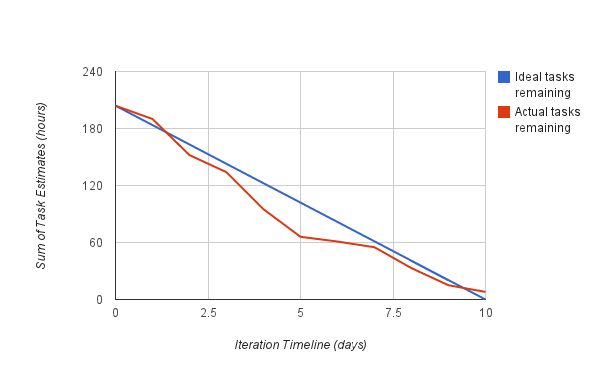
\includegraphics[width=15cm]{Pictures/Charts/Sprint4burndown}
	\end{center}
	\caption{Sprint 4 burndown chart}
	\label{fig:sprint4burndown}
\end{figure}

 \begin{table}
 	\begin{center}
 	\begin{sideways}
 		\begin{tabular}{|l | p{7.5cm} | c | c | c | c | l |}
 			\hline
 			  \#  ID 	& Task 	& Story points 	& Estimated & Actual &
 			  Estimated Left & Responsible \\
 			\hline
 			1.1 & View for amount of stars collected & 1 & 4 & 4 & 0 & Yngve\\
 			\hline
 			1.2 & Connect reward view to the database & 1 & 4 & 3 & 0 & Yngve\\
 			\hline
 			2.1 & Refine the distraction for the children & 3 & 12 & 10 & 0 & Yngve\\
 			\hline
 			3.1 & Finalize instructions for children & 3 & 12 & 10 & 2 & Aleks\\
 			\hline
 			4.1 & Make solution for registering a treatment & 3 & 12 & 7 & 0 & Esben\\
 			\hline
 			4.2 & Implement pollenfeed to log & 10 & 40 & 6 & 0 & Esben\\
 			\hline
 			4.3 & Finalize view for showing pollen and medications taken at a given day & 2 & 8 & 5 & 0 & Esben\\
 			\hline
 			5.1 & Finalize instruction for medications & 3 & 12 & 7 & 2 & Aleks\\
 			\hline
 			6.1 & Make view for viewing existing medication plans & 4 & 16 & 16 & 0 & Eirik\\
 			\hline
 			6.2 & Import medication list from database to medication plan settings & 1 & 4 & 1 & 0 & Esben\\
 			\hline
 			6.3 & Improve layout for making medication plan & 2 & 8 & 10 & 2 & J\o rgen\\
 			\hline
 			6.4 & Save the medication plan to the database & 3 & 12 & 6 & 0 & J\o rgen\\
 			\hline
 			7.1 & User interface for changing reminder preferences & 1 & 4 & 0 & 4 & -\\
 			\hline
 			7.2 & Secure that the reminder is giving alarms independently of internet connection and sound level on phone & 1 & 4 & 8 & 0 & Eirik \\
 			\hline
 			8.1 & Create web interface for adding medical plan doses & 1 & 4 & 1 & 0 & Yngve \\
 			\hline
 			8.2 & Create web interface for removing medical plan doses & 1 & 4 & 1 & 0 & Yngve \\
 			\hline
 			8.3 & Create web interface for getting log grouped on days & 1 & 4 & 1 & 0 & Yngve \\
 			\hline
 			9.1 & Refine Karotz app manus, after feedback from customer & 3 & 12 & 13 & 2 & Yngve \\
 			\hline
 			9.2 & Record new voice messages for the Karotz & 1 & 4 & 2 & 0 & Yngve \\
 			\hline
 			10.1 & Refine design for registering treatment & 1 & 4 & 8 & 0 & Esben and J\o rgen \\
 			\hline
 			10.2 & Refine design for instructions & 2 & 8 & 6 & 0 & Esben \\
 			\hline
 			10.3 & Refine GUI for the main menu & 1 & 4 & 3 & 0 & Aleks and Esben \\
 			\hline
 			11.1 & Refine alarm and distraction regarding database calls & 2 & 8 & 3 & 4 & Yngve \\
 			\hline 
 			\bfseries{SUM} & & \bfseries{51} & \bfseries{204} & \bfseries{131} & \bfseries{16} & \\
 			\hline
 		\end{tabular}
 	\end{sideways}
 	\caption{Sprint Retrospective, Sprint 4}
 	\label{tab:sprint4burndown}
 	\end{center}
\end{table}

Figure \ref{fig:sprint4burndown} and table \ref{tab:sprint4burndown} show the burndown chart for the fourth 
sprint. From the burndown chart, the fourth sprint looks like a success. Ahead of the 
sprint, the function number for the story points was lowered, since we expected to work faster. 
This was done independently of our estimation, to not make biased results. The team worked faster 
than expected on a general base. Some tasks were still overestimated. The reason for this was 
little knowledge towards the task and how it should be solved. For example the implementation of the 
pollen feed proved to be much faster than expected, since we hardcoded the values. 

The sprint contained 204 estimated work hours, and our goal was to complete 175 of those, which correspons
to $175/4=43.75$ story points with our base multiplier of 4. While only 131 work hours were recorded, there
were only 16 estimated work hours left when the sprint was over. This corresponds to $16/4=4$ story points.
Therefore, we completed $51-4=47$ story points, which is $47-43.75=3.25$ more than our goal. The sprint was 
therefore considered a success with a satisfactory result.